%1. Grundlagen
\chapter{Grundlagen}
Diese Studienarbeit befasst sich mit dem komplexen Thema der Elliptischen Kurven in der Kryptographie. Die Kryptographie ist ein mathematisches Thema, bei welchem es zu Anfang der Legung einer Grundlage für das Verständnis der Inhalte dieser Studienarbeit bedarf. In diesem Kapitel werden sowohl die mathematischen als auch die kryptographischen Grundlagen zum Verständnis der Inhalte dieser Studienarbeit gelegt.

\section{Primzahlen}
In der Zahlentheorie, einem Teilbereich der Mathematik, werden viele unterschiedliche Eigenschaften von Zahlen untersucht. Durch die Untersuchung erhofft man sich neue Erkenntnisse für Wissenschaft und Technik. Die Primzahlen als mathematisches Forschungsgebiet sind hierbei ein Teilbereich der Zahlentheorie. Im Folgenden werden Primzahlen definiert und deren Eigenschaften erläutert. Anschließend wird untersucht, wie Primzahlen berechnet werden können. Am Ende wird erläutert, welche Rolle Primzahlen in der Kryptologie und modernen Kryptosystemen innehaben.

\subsection{Definition und Eigenschaften}
Es gibt viele unterschiedliche Zahlenmengen. Beispielsweise gibt es die Menge der reellen Zahlen $\mathbb{R}$. Diese beinhalten als Teilmenge die rationalen und die irrationalen Zahlen. Die natürlichen Zahlen $\mathbb{N}$ bilden hierbei alle positiven ganzen Zahlen ab. Dabei gibt es $\mathbb{N^{+}}$ exklusive der Zahl 0 als Teilmenge mit $\mathbb{N^{+}} = \{1, 2, 3, 4, ..., \infty\}$ und $\mathbb{N}_0$ inklusive der Zahl 0 als Teilmenge mit $\mathbb{N}_0 = \{0, 1, 2, 3, 4, ..., \infty\}$. Die Primzahlen $\mathbb{P}$ sind hierbei etwas ganz besonderes. Sie unterscheiden sich von anderen Zahlen. Sie sind eine Teilmenge der natürlichen Zahlen und die Kardinalität ihrer Elemente ist unendlich respektive die Anzahl der Primzahlen ist unendlich. Die Unendlichkeit der Primzahlen konnte schon mit mehreren mathematischen Sätzen bewiesen werden, unter anderem dem Satz von Euklid. Auf die unendlichkeit der Primzahlen sowie deren bestimmung wird später in \ref{sec:bestimmung_primzahlen} eingegangen.\\

Doch wie genau sind Primzahlen definiert? Dafür muss man erst geklärt werden, was zusammengesetzte Zahlen sind. Dadurch können die Primzahlen klarer von anderen natürlichen Zahlen abgegrenzt werden. Eine natürliche Zahl mit n $\geq$ 2 ist eine zusammengesetzte Zahl, falls es zwei natürliche Zahlen m und k mit den Eigenschaften m, k $\geq$ 2 und m, k $\neq$ n gibt, für die gilt: $m \cdot k = n$. Natürliche Zahlen können also immer als Produkt zweier natürlicher Zahlen beschrieben werden. Primzahlen bilden hierzu das Gegenstück. Eine Primzahl p ist eine natürliche Zahl mit p $\geq$ 1, wobei p nur durch 1 und sich selbst teilbar sein darf. Durch diese Eigenschaft sind Primzahlen nicht das Produkt von natürlichen Zahlen und können somit nicht durch Multiplikation gebildet werden. Nimmt man als Beispiel die natürliche Zahl 28. Sie kann durch Multiplikation aus den Zahlen 2 und 14 gebildet werden: $2 \cdot 14=28$. Die Primzahl 7 hingegen lässt sich nicht als Produkt von natürlichen Zahlen darstellen.\\

Eine weitere Eigenschaft von Primzahlen ist, dass sie das Grundgerüst zur Bildung von Zahlen sind, da man aus ihnen alle anderen natürlichen Zahlen bilden kann. Eine natürliche Zahl n mit n $\geq$ 2 kann wie bereits beschrieben immer als Produkt von (mindestens) zwei weiteren natürlichen Zahlen dargestellt werden. Jede natürliche Zahl kann in ihre Primfaktoren zerlegt werden. Dies nennt man Primfaktorzerlegung. Dadurch ist die Zahl als Produkt von mehreren Primzahlen dargestellt. Nehmen wir als Beispiel die Zahl 28. Vorhin stellten wir dies durch die Multiplikation von 2 und 14 dar: $2 \cdot 14=28$. Die Zahl 2 ist eine Primzahl. Die Zahl 14 ist noch nicht in ihre Primzahlfaktoren zerlegt. Sie lässt sich als folgendes Produkt darstellen: $2 \cdot 7=14$. Da 7 auch eine Primzahl ist, wurden alle Primfaktoren gefunden. Die Zahl 28 lässt sich in ihrer Primfaktorzerlegung also wie folgt darstellen: $2 \cdot 2 \cdot 7=28$. Die Mehrfachheit von Primzahlen lässt sich auch als Potenz schreiben. Somit wird daraus $2^{2} \cdot 7=28$. Der Vorteil durch die Potenzen zeigt sich besonders bei großen Zahlen, da diese oft eine große Anzahl an Primfaktoren haben können. Nimmt man als Beispiel die Zahl 5281250000. Diese setzt sich mit ihren Primfaktoren wie folgt zusammen: $2 \cdot 2 \cdot 2 \cdot 2 \cdot 5 \cdot 5 \cdot 5 \cdot 5 \cdot 5 \cdot 5 \cdot 5 \cdot 5 \cdot 5 \cdot 13 \cdot 13=5281250000$. Man erkennt rasch, dass sich die Primfaktoren mit der Potenzschreibweise zusammenfassen lassen und man so die Primfaktorzerlegung wie folgt darstellen kann: $2^{4} \cdot 5^{9} \cdot 13^{2}=5281250000$. Die Vorteile der Potenzschreibweise liegt hier auf der Hand, da man erheblich Zeit beim Aufschreiben und Platz auf dem Papier spart.

\subsection{Bestimmung von Primzahlen}\label{sec:bestimmung_primzahlen}
x

\begin{figure}[!h]
\centering
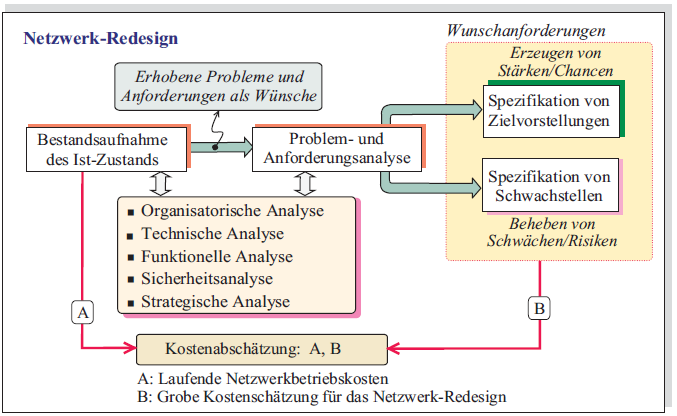
\includegraphics[width=\textwidth]{grafiken/aufgaben_redesign.png}
\caption[Hauptaufgaben der Ist-Analyse beim Redesign einer Netzwerkinfrastruktur]{Hauptaufgaben der Ist-Analyse beim Redesign einer Netzwerkinfrastruktur \\ Quelle: \cite{Berghammer.2021}}
\label{fig:aufgaben_redesign}
\end{figure}

\subsection{Rolle der Primzahlen in der Kryptologie}
x

\section{Algebraische Strukturen}
Definiert durch die Zahlentheorie und als zentraler Untersuchungsgegenstand des mathematischen Teilgebietes der universellen Algebra, liefern algebraische Strukturen die Basis zur Realisierung komplexer symmetrischer und asymmetrischer Kryptosysteme, weshalb wir im folgenden Kapitel die Eigenschaften relevanter algebraischer Strukturen näher betrachten wollen. Darüber hinaus möchten wir Ihnen auch einige Werkzeuge zum Rechnen in der jeweiligen algebraischen Struktur an die Hand geben, welche zur späteren Realisierung von Kryptosystemen benötigt werden.\\

Unter einer sehr allgemeinen Betrachtung ist eine mathematische Struktur eine Liste nichtleerer Mengen, genannt Trägermengen, mit Elementen aus den Trägermengen, genannt Konstanten, und mengentheoretischer Konstruktionen über den Trägermengen. Diese sind konkret Funktionen über den Trägermengen.
Im Weiteren beschränken wir uns auf den Fall einer einzigen Trägermenge, wodurch die Strukturen als homogen bezeichnet werden können.
\paragraph{Definition: Homogene algebraische Struktur}
Eine homogene algebraische Struktur ist ein Tupel $(M,c_1,\dots,c_m,f_1,\dots,f_n)$ mit $m,n \in \mathbb{N}$ und $n \geq 1$. Dabei ist $M$ eine nichtleere Menge, genannt \textbf{Trägermenge}, alle $c_i$ sind Elemente aus $M$, genannt die \textbf{Konstanten}, und alle $f_i$ sind $s_i$-stellige Funktionen $f_i:M \rightarrow M$ im Fall $s = 1$ und $f_i:M^{s_i} \rightarrow M$ im Fall $s_i>1$, genannt die (inneren) \textbf{Operationen}. Die lineare Liste$(0,\dots,0,s_1,\dots,s_n)$ mit $m$ Nullen heißt \textbf{Typ} oder die \textbf{Signatur}.\newline

Laut dieser Definition muss eine homogen algebraische Struktur nicht unbedingt Konstanten enthalten, jedoch mindestens eine Operation. Das Paar $(\mathbb{N},+)$ bildet beispielsweise eine homogene algebraische Struktur des Typs (2). Das 5-Tupel $(\mathbb{N},0,1,+,\cdot)$ bildet ebenfalls eine homogen algebraische Struktur des Typs (0,0,2,2).

Algebraische Strukturen unterscheiden sich grundsätzlich durch ihren Typ. Wirklich charakterisiert werden sie aber erst durch die jeweils geltenden Axiome, d.h. bestimmte Eigenschaften, welche für die Konstanten und Operationen gefordert werden. Durch die Hinzunahme immer weiterer Axiome, entsteht eine Hierarchie immer feinerer Strukturen, an deren Anfang der Monoid steht.

\subsection{Monoid}
\paragraph{Definition: Monoid}
Eine algebraische Struktur $(M,e,\cdot)$ des Typs (0,2) heißt ein Monoid, falls für alle $x,y,z\in M$ die folgenden Monoid Axiome gelten: 
\begin{itemize}
\item (Ass) $x \cdot (y \cdot z) = (x \cdot y) \cdot z$
\item (Neu) $e \cdot x = x = x \cdot e$
\end{itemize}  Gilt zusätzlich noch für alle $x,y \in M$ die Gleichung $x \cdot y = y \cdot x$, so heiß $(M,e,\cdot)$ ein \textbf{kommutatives Monoid}.\\

Die erste und die letzte Gleichung bilden das Assoziativ- und Kommutativgesetz ab. Durch die mittlere Gleichung wird ein neutrales Element $e$ bezüglich der Operation gefordert, wobei sowohl die \textbf{Linksneutralität} als auch die \textbf{Rechtsneutralität} spezifiziert wird.\\

Einfache Beispiele für Monoide sind $(\mathbb{N},0,+)$, $(\mathbb{N},1,\cdot)$ und $(\mathbb{Z},0,+)$. Die  Potenzierung in solchen Monoiden ist folgendermaßen definiert.
\paragraph{Definition: Potenzierung}
In einem Monoid $(M,e,\cdot)$ definiert man die $n$-te \textbf{Potenz} $x^n$ von $x \in M$ durch $x^0 := e$ und $x^{x+1} = x \cdot x^n$ für alle $n \in \mathbb{N}$.\\

Daraus ergibt sich für den Monoid $(\mathbb{N},1,\cdot)$ die aus $\mathbb{R}$ gewohnte Potenzierung. Nach welcher für ein $x \in \mathbb{N}$ die Potenzierung $x^n = x_1 \cdot x_2 \cdot \dots \cdot x_n$ ergibt. Betrachtet man jedoch den Monoid $(\mathbb{N},0,+)$, so ergibt analog dazu für ein $x \in \mathbb{N}$ die Potenzierung $x^n = x_1 + x_2 + \dots + x_n = x \cdot n$, was also einer Multiplikation von $x$ mit $n$ entspricht.

\subsection{Gruppe}
\paragraph{Definition: Gruppe}
Eine algebraische Struktur $(G,e,\cdot,inv)$ des Typs $(0,2,1)$ heißt \textbf{Gruppe}, falls für alle $x,y,z \in G$ die folgenden Axiome gelten:

\begin{itemize}
\item (Ass)	$x \cdot (y \cdot z) = (x \cdot y) \cdot z$
\item (Neu)	$e \cdot x = x$$ $$inv(x) \cdot x = e$
\item (Inv)	$inv(x) \cdot x = e$
\end{itemize}

Gilt wiederum die Gleichung $x \cdot y = y \cdot x$ für alle $x,y \in G$, so heißt $(G,e,\cdot,inv)$ eine \textbf{kommutative Gruppe}.

\subsection{Ring}
\subsection{Körper}

\section{Allgemeines zur Verschlüsselung}
XXX

\subsection{Symmetrische und Asymmetrische Verschlüsselung}
x

\subsection{Diffie-Hellmann}
x

\section{Ziel der Arbeit}
XXX

\section{Geplante Vorgehensweise}
XXX